\subsection{Формирование набора данных}
\label{sec:impl_dataset}
    Набор данных формируется на основе заранее собранной и предподготовленной информации.
    Информация собирается определённый, фиксированный отрезок времени.
    Для формирования набора данных использовалась информация собранная с 06.04.2016 по 17.04.2016.
    Было получено множество, основные характеристики которого приведены в таблице~\ref{tabular:dataset_desc}.
    \begin{table}[ht!]
        %\small
        \caption{Сводная характеристика по собранному множеству твитов и новостей за период с 06.04.2016 по 17.04.2016\bigskip}
        \centering

        \label{tabular:dataset_desc}
        \begin{tabular}{|p{8cm}|c|}
            \hline
            \bf{\specialcell{Метрика}} &
            \bf{\specialcell{Значение}} \\ \hline

            Количество твитов & 495552 \\ \hline
            Количество новостей & 13711 \\ \hline
            Количество твитов, содержащих ссылку & 150510 \\ \hline
            Количество уникальных ссылок, встречаемых в твитах & 101017 \\ \hline
            Количество твитов, содержащих ссылку на новости из рассматриваемых новостных источников & 4324 \\ \hline
            Количество уникальных ссылок на новости из рассматриваемых новостных источников & 2979 \\ \hline
        \end{tabular}
    \end{table}
    В дальнейшей под собранными данными будет подразумеваться описанное в таблице~\ref{tabular:dataset_desc} множество.

    Для построения требуемого в работе набора данных необходимо найти множество связей твит-новость.
    Процесс поиска связей твит-новость называется \textit{разметкой набора данных}. В работе используется два способа разметки:
    \begin{enumerate}
        \item автоматическая разметка набора данных;
        \item ручная разметка набора данных.
    \end{enumerate}

    В результате разметки будет получаться некоторое количество пар твит-новость, в которых твит, практически полностью будет совпадать с заголовком новости.
    Будем в дальнейшем называть такие связи твит-новость, в которых менее половины слов из твита не встречаются в заголовке статьи \textit{тривиальными}.

    \subsubsection{Автоматическое разметка набора данных}
        Автоматически построенный набор данных состоит из всех собранных новостей и твитов, которые содержат ссылку на одну из собранных новостей.
        Получаем множество состоящее из 4324 твитов, 13711 новостей, а также 4324 связей между ними.

        Проанализируем полученный набор данных, нас интересует насколько в парах твит-новость, твит отличается от соответсутющей новости.
        Для этого для каждого твита берём его текст, для каждой новости берём заголовок.
        Все тексты поэтапно преобразовали согласно алгоритму, который сопоставляет тексту множество слов и состоит из следующей последовательность действий:
        \begin{enumerate}
            \item текст конвертируется в формат unicode;
            \item текст разбивается на токены;
            \item полученное множество токенов очищается от токенов, не являющихся словами;
            \item из множества удаляются все слова входящие в словарь стопслов;
            \item из множества удаляются все дубли.
        \end{enumerate}
        На основе предподготовленных данных для каждой пары твит, связанная с твитом новость измерялось две метрики:
        длина пересечения слов твита и слов новости, нормализованная по длине новости;
        количество слов в твите, которые не встречаются в новости.

        На рисунке~\ref{pic:auto_histogram} изображена зависимость количества пар твит-новость от длины пересечения слов твита и слов новости, нормализованной по длине новости.
        \begin{figure}[h!]
            \center
            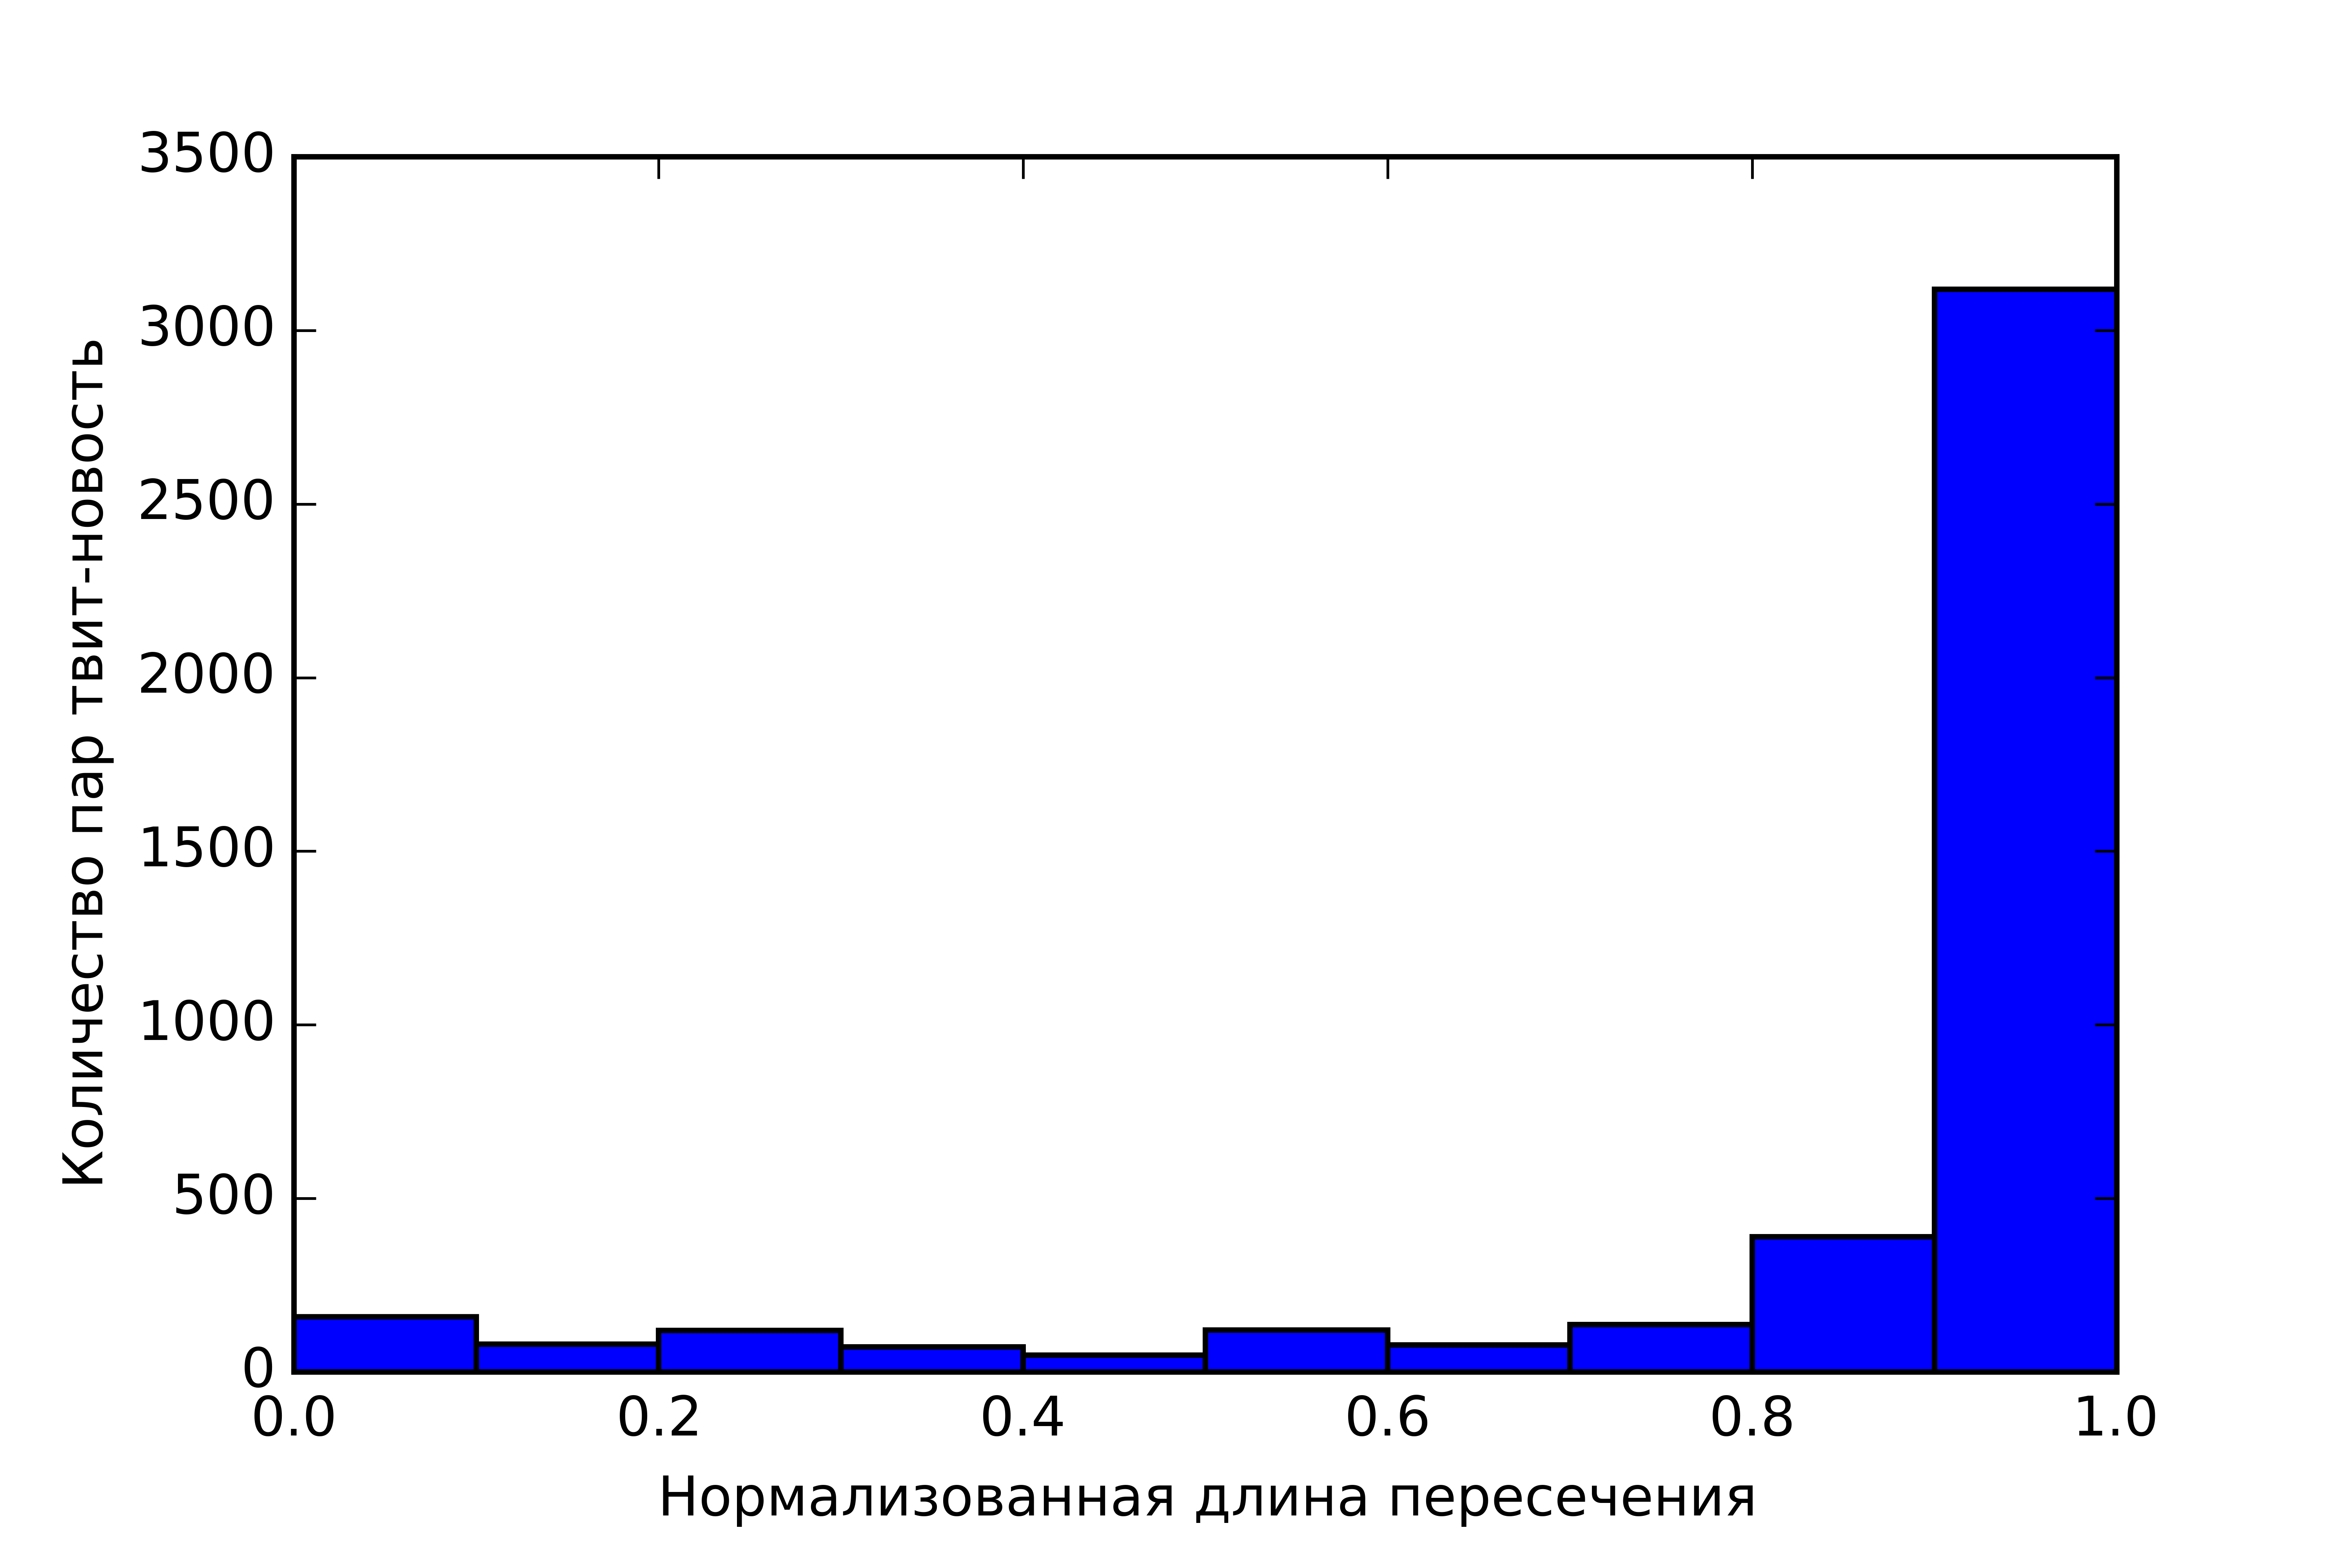
\includegraphics[scale=0.85]{dataset_auto_normalized_intersect_histogram.png}
            \caption{Зависимость количества пар твит-новости от нормализованный длины пересечения множества слов (автоматически размеченный набор данных).}
            \label{pic:auto_histogram}
        \end{figure}
        Как видно из рисунка~\ref{pic:auto_histogram} слова в подавляющем большинстве твитов полностью совпадают со словами в соответствующей новости.
        Среди 4324 пар твит-новость в 3082 парах твит полностью совпадает с заголовком новости. Остаётся 1242 пар, которые не являются просто копией заголовка, среди этих пар
        нас интересуют те, в которых твит не является обрезанной частью заголовка статьи.

        Для выявления количества пар, где твит содержит информацию не содержащуюся в заголовке статьи посмотрим на зависимость количества пар твит-новость от процента уникальных слов в твите,
        эта зависимость изображена на рисунке~\ref{pic:auto_percent}.
        \begin{figure}[h!]
            \center
            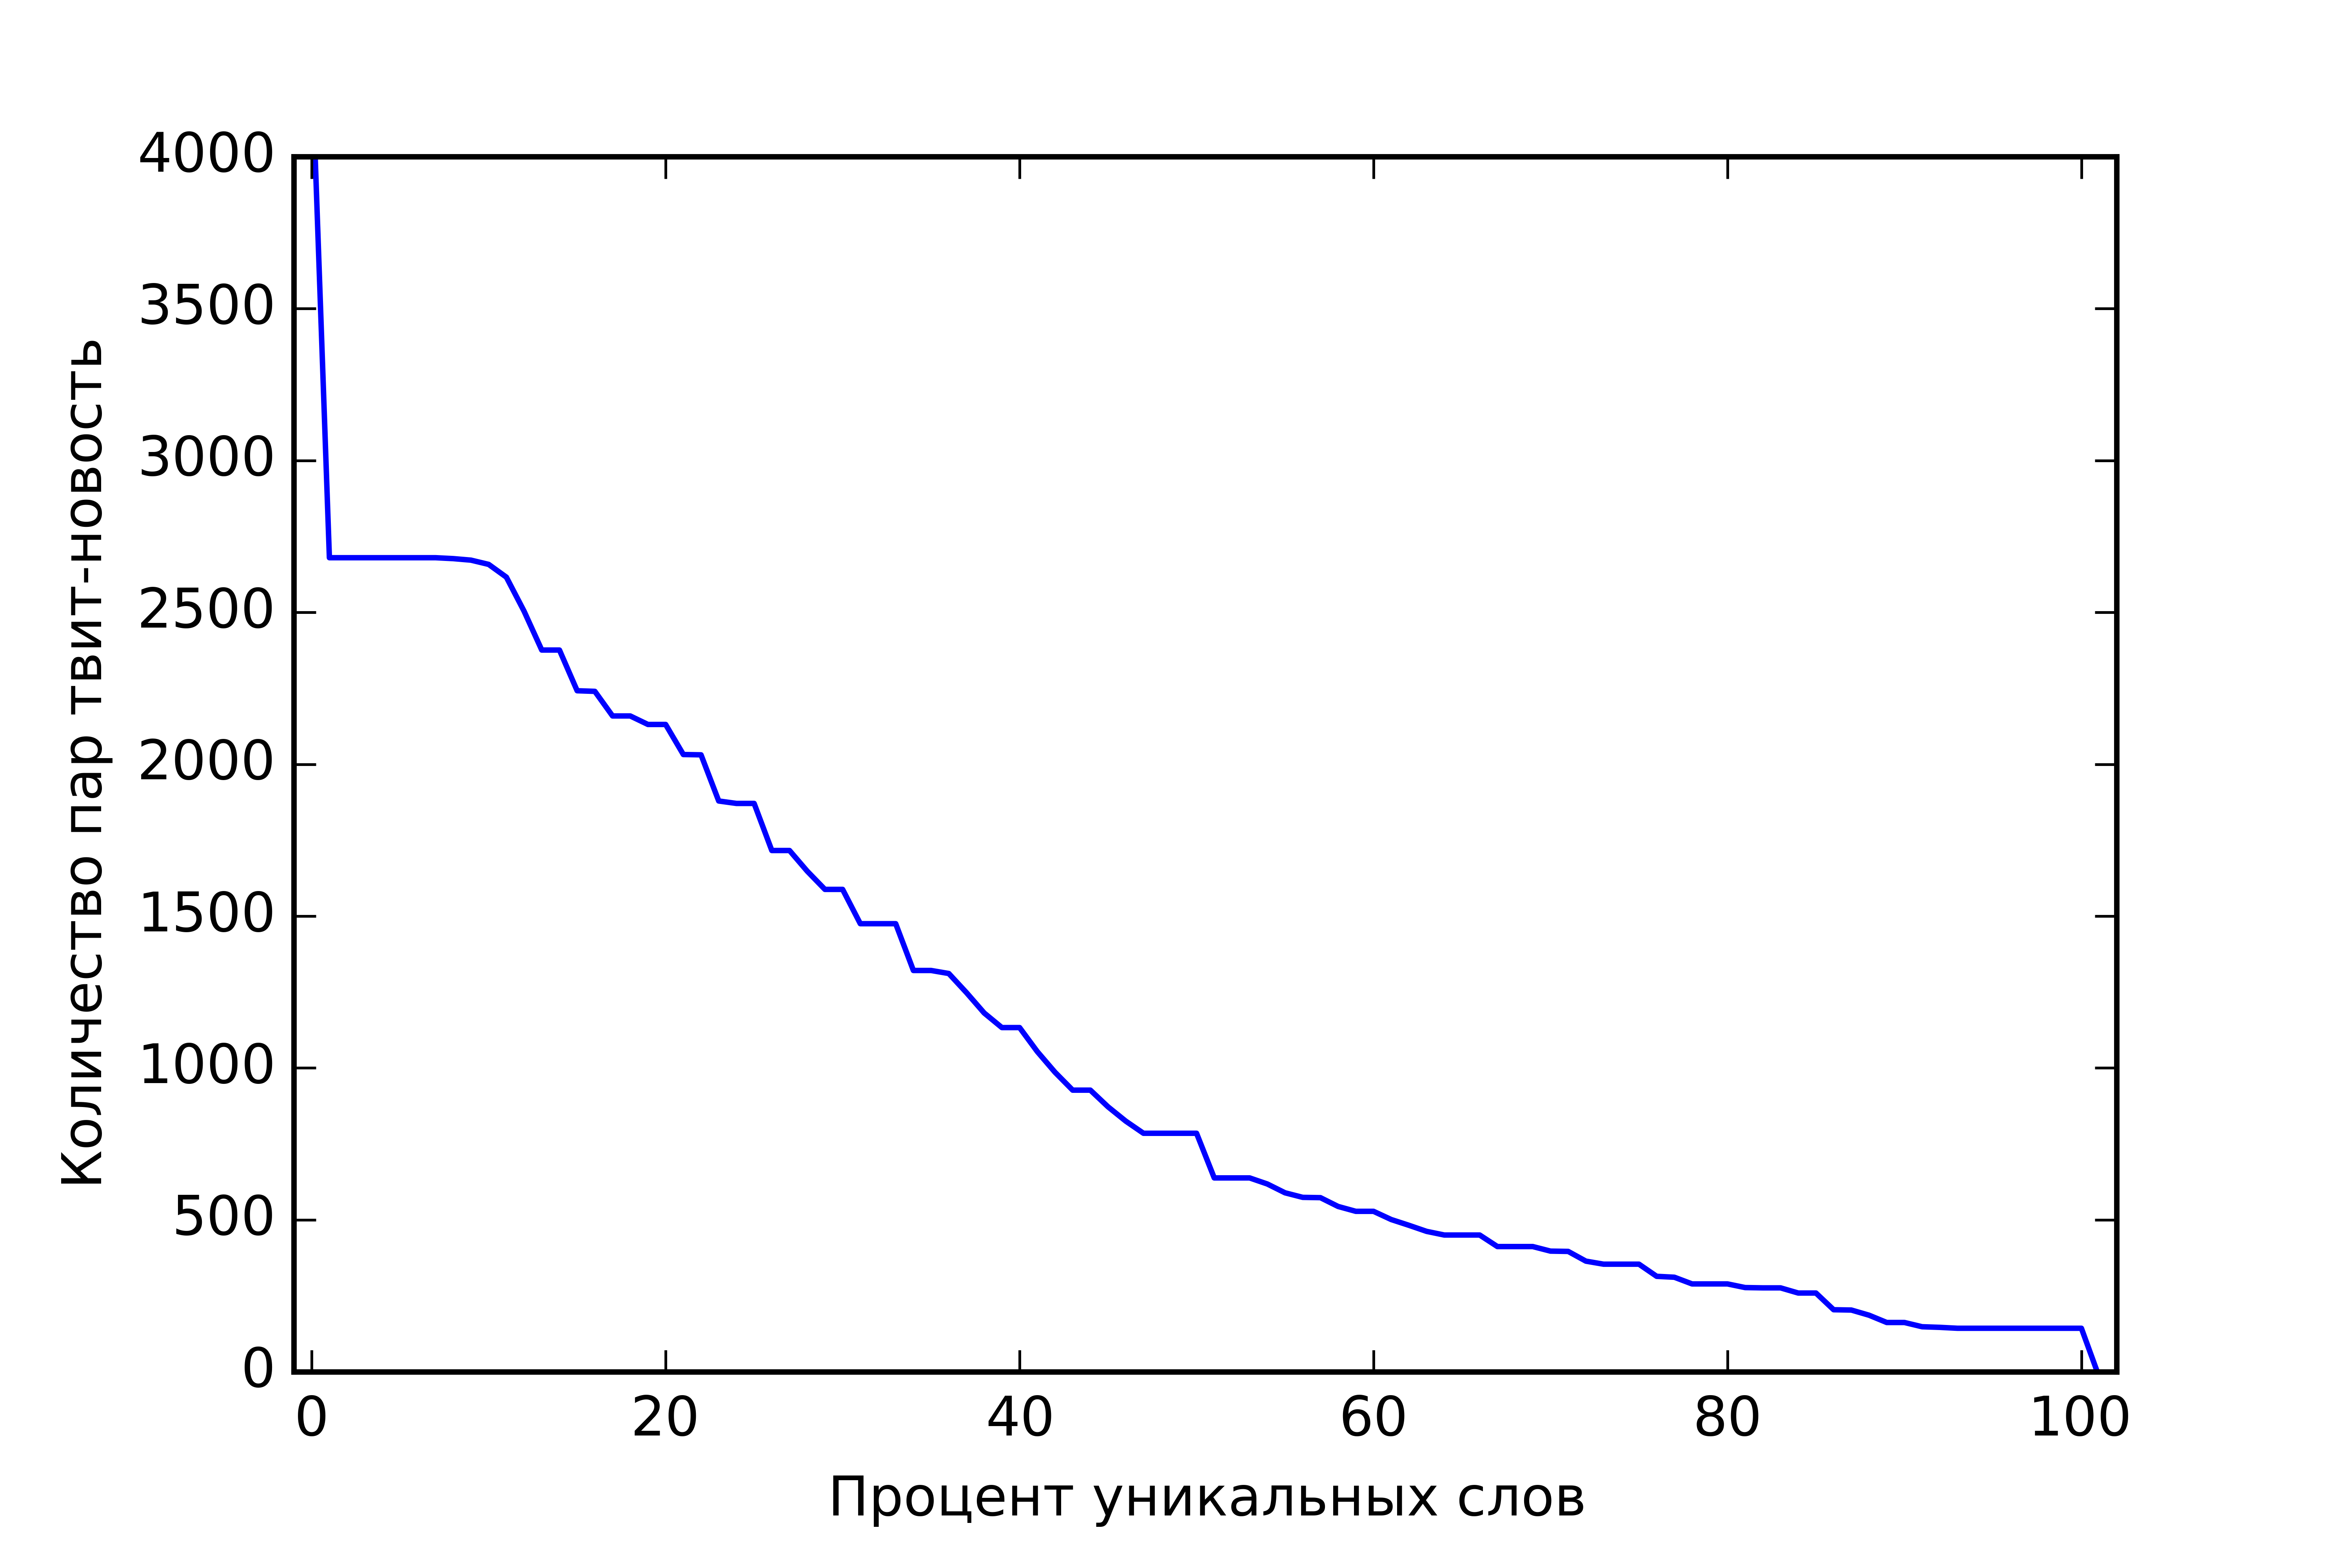
\includegraphics[scale=0.85]{dataset_auto_unique_words_percent.png}
            \caption{Зависимость количества пар твит-новости от процента уникальных слов в твите (автоматически размеченный набор данных).}
            \label{pic:auto_percent}
        \end{figure}
        Как видно из рисунка~\ref{pic:auto_percent} количество твитов более с чем половиной уникальных слов достаточно мало.

        На основе исследования зависимости можно получить грубую оценку количества нетривиальных связей.
        В исследуемом наборе данных таких связей порядка 500-1000, что очень мало и составляет примерно 12-23\% от общего числа пар.

    \subsubsection{Ручная разметка набор данных}
        Для получения большего количества нетривиальных пар твит-новость была предпринята ручная разметка набора данных.
        Для ручной разметки необходимо предподготовить данные. Основные этапы предподготовки данных:
        \begin{enumerate}
            \item на основе множества новостей строится список именованных сущностей $L$;
            \item случайным образом берётся подмножество $T$ множества твитов;
            \item из полученного множества $T$ удаляются все твиты, которые удолетворяют следующим правилам:
            \begin{enumerate}
                \item твит является ретвитом,
                \item твит содержит ссылку на URL с плохим доменным именем (под \textit{плохим} доменным именем подразумевается доменное имя,
                которое достаточно популярно и не ведёт на новостной источник, в работе использовался следующий список плохих доменных имён:\
                \url{apps.facebook.com}, \url{ask.fm}, \url{twitter.com}, \url{apps.facebook.com}, \url{www.instagram.com}, \url{vk.cc}),
                \item в приведённом к нормальной форме~(определение нормальной формы находится в главе\ref{subsubsec:lemma}) тексте твита содержится менее 2 слов из списка именованных сущностей $L$;
            \end{enumerate}
            \item c помощью метода определения схожести текстов на основе частотности употребления слов каждому твиту сопоставляется 10 наиболее схожих с ним новостей.
        \end{enumerate}
        В качестве результата предподготовки получается множества пар твит-ранжированный список новостей.

        Предподготовленные данные размечаются экспертом.
        Разметка заключается в записи специальной отметки рядом с подходящей новости из предложенного списка для каждого твита.
        Для каждого твита отмечается только одна, наиболее подходящая новость, или не отмечается ни одной.

        Было сформировано множество из 7373 пар твит-ранжированный список новостей. В нём экспертом было выявлено 1600 связей твит-новость.
        Получаем набор данных, состоящий из 1600 твитов, 13711 новостей, а также 1600 связей между ними.

        Для сравнения вручную построеннго набора данных с набором данных, полученным автоматически были построены две зависимости~---~
        зависимость количества пар твит-новость от длины пересечения слов твита и слов новости и  зависимость количества пар твит-новости от процента уникальных слов в твите.
        На рисунке~\ref{pic:manual_histogram} изображена зависимость количества пар твит-новость от длины пересечения слов твита и слов новости, нормализованная по длине новости.
        \begin{figure}[h!]
            \center
            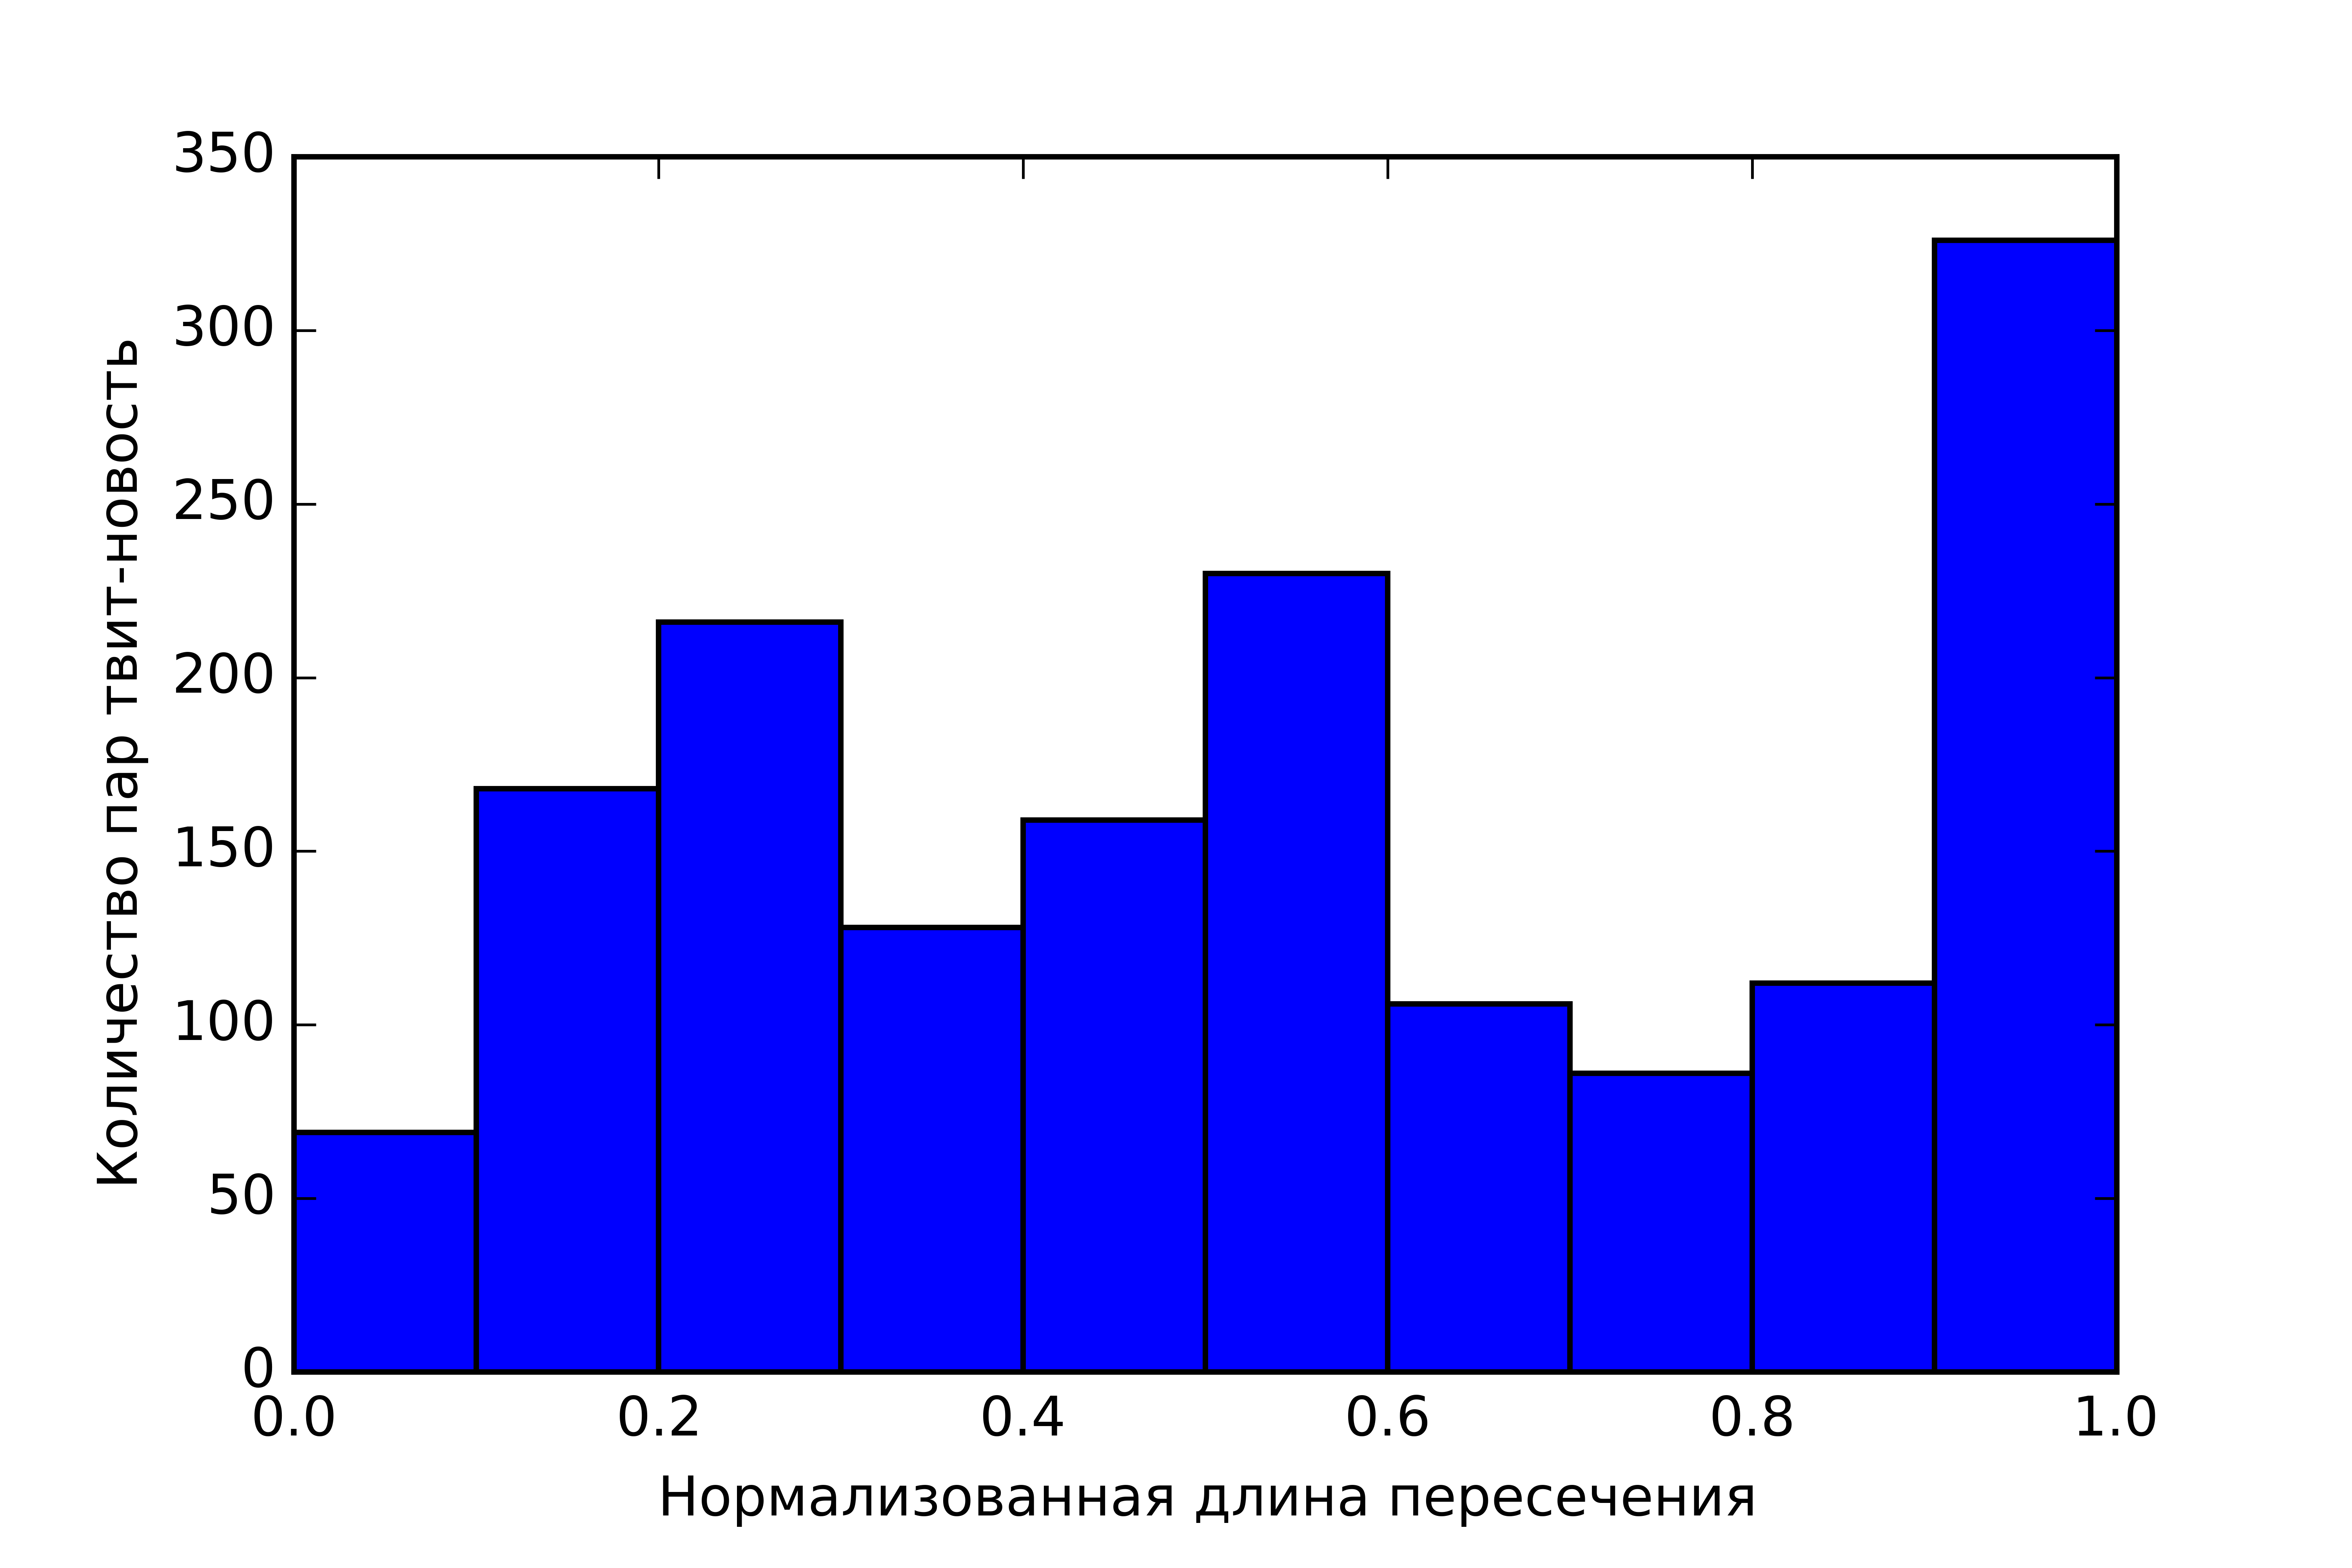
\includegraphics[scale=0.85]{dataset_manual_normalized_intersect_histogram.png}
            \caption{Зависимость количества пар твит-новости от нормализованный длины пересечения множества слов (вручную размеченный набор данных).}
            \label{pic:manual_histogram}
        \end{figure}
        Как видно из рисунка~\ref{pic:manual_histogram} было получено распределение намного более близкое к равномерному, чем в случае автоматически размеченного набора данных.

        На рисунке~\ref{pic:manual_percent} изображена зависимость количества пар твит-новость от процента уникальных слов в твите.
        \begin{figure}[h!]
            \center
            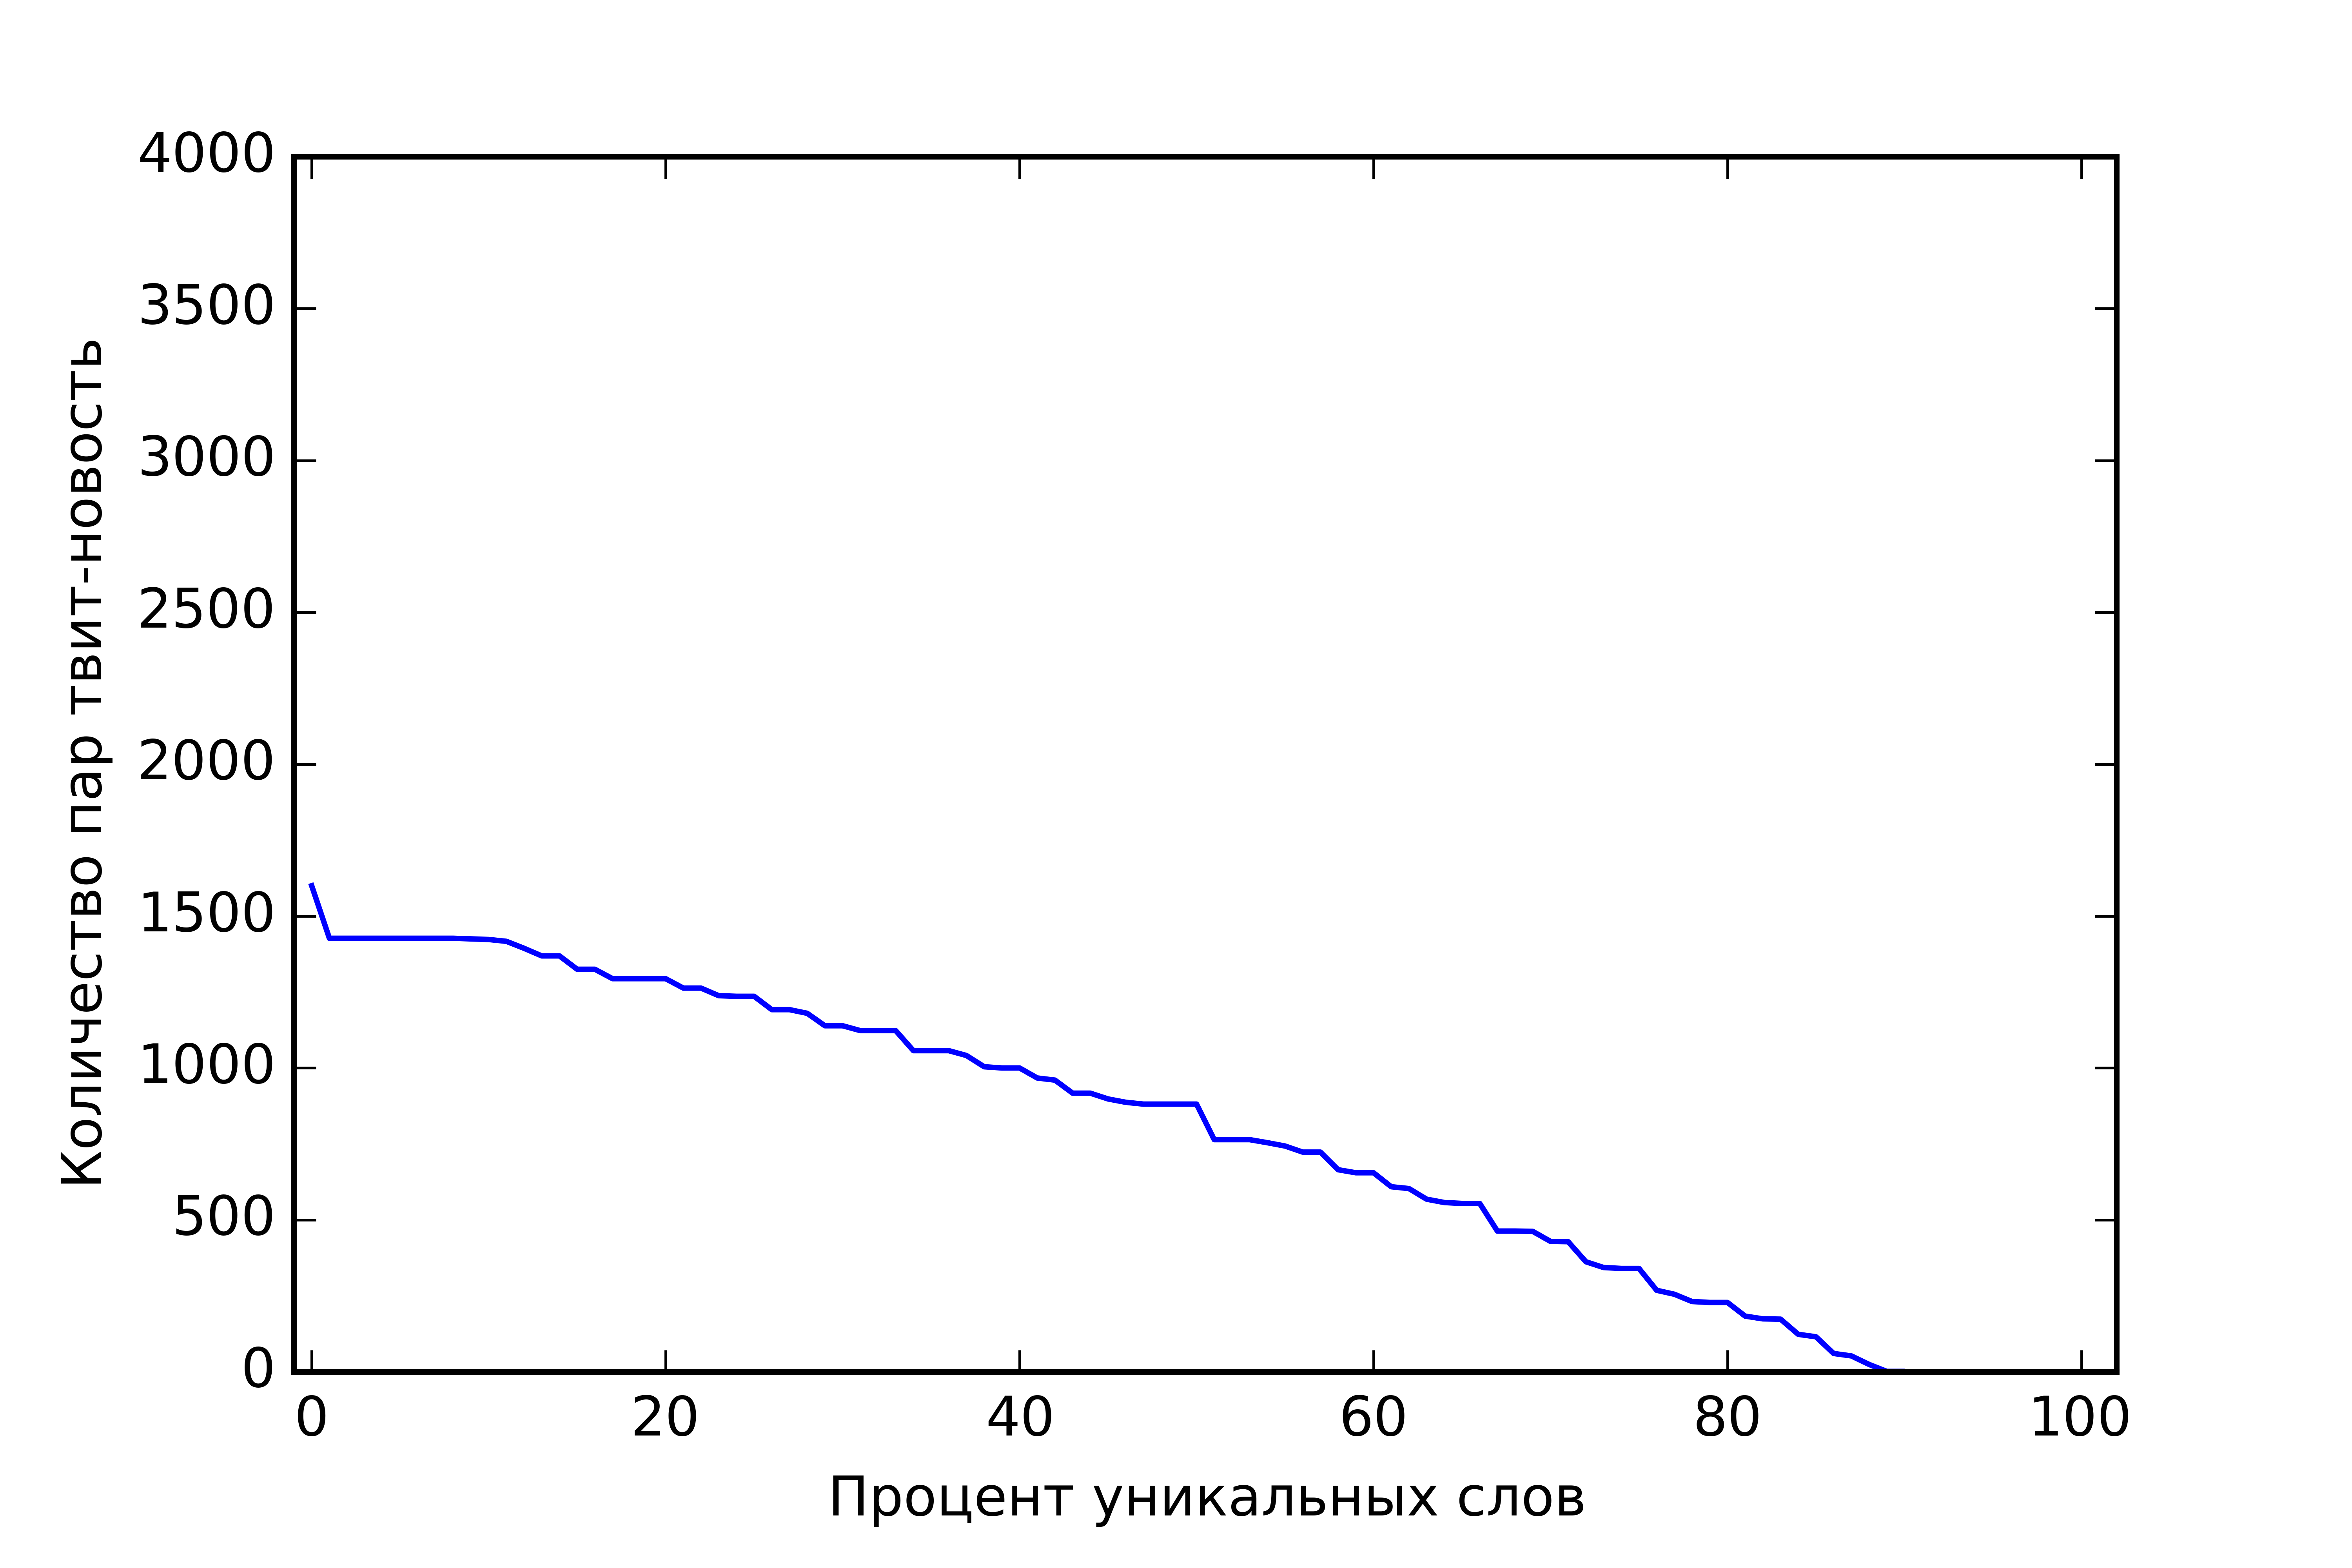
\includegraphics[scale=0.85]{dataset_manual_unique_words_percent.png}
            \caption{Зависимость количества пар твит-новости от процента уникальных слов в твите (вручную размеченный набор данных).}
            \label{pic:manual_percent}
        \end{figure}
        Как видно из рисунка~\ref{pic:manual_percent} количество твитов более с чем половиной уникальных слов сравнимо с аналогическим количеством в автоматически размеченном наборе данных,
        несмотря на то, что автоматически размеченный набор данных почти в три раза больше, чем вручную размеченный набор данных.

        Количественные значение полученных метрик приведены в таблице~\ref{tabular:dataset_stat}.
        \begin{table}[ht!]
            %\small
            \caption{Сравнение количества твитов \bigskip}
            \centering

            \label{tabular:dataset_stat}
            \begin{tabular}{|p{5cm}|c|c|}
                \hline
                \bf{\specialcell{Метрика}} &
                \bf{\specialcell{Автоматически размеченный \\ набор данных}} &
                \bf{\specialcell{Вручную размеченный \\ набор данных}} \\ \hline

                Количество связей & 4324 & 1600 \\ \hline
                Количество нетривиальных связей & 785 & 881 \\ \hline
                Процент нетривиальных связей от общего числа связей~(\%) & 18.15  & 55.06 \\ \hline
            \end{tabular}
        \end{table}
        Как видно из таблицы \ref{tabular:dataset_stat} вручную собранный набор данных намного более качественный, чем автоматический.
        Но как в ручном, так и в автоматическом наборе данных содержится очень мало нетривиальных связей твит-новость (в сравнении с количеством новостей).

    \subsubsection{Построение связей текст-текст}
        всё о построение этих связей, \textcolor{red}{написать после написания review}

    \subsubsection{Сформированные датасеты}
        На основе данных собранных за период ... было сформировано несколько эталонных наборов, а именно:
        \begin{enumerate}
            \item
        \end{enumerate}
        Ключевая информация характеризующая эталонные наборы представлена в таблице~\ref{tabular:dataset_info}

        \begin{table}[ht!]
            %\small
            \caption{Сводная таблица по эталонным наборам данных\bigskip}
            \centering

            \label{tabular:tau_PP}
            \begin{tabular}{|p{8cm}|c|c|c|}
                \hline
                \bf{\specialcell{Описание набора данных}} &
                \bf{\specialcell{Рабочее \\ название}} &
                \bf{\specialcell{Количество \\ твитов}} &
                \bf{\specialcell{Количество \\ новостей}} \\ \hline
                Набор данных с вручную размеченными связями & manual & 1600 & 13711 \\ \hline
                Набор данных с автоматически размеченными связями & auto & 4324 & 13711 \\ \hline
                Набор данных с состоящий из объединения всех размеченных связей& total & 5798 & 13711 \\ \hline
                Набор данных с состоящий из объединения всех размеченных связей, с количеством новостей нормализованным относительно количества твитов & total\_cutted & 5798 & 6011 \\ \hline
            \end{tabular}
        \end{table}





        список из всех сформированных датасетов с описанием каждого из них

